\documentclass{article}

\usepackage{graphicx}
\usepackage{tikz}
\usepackage{tikzsymbols}
\usetikzlibrary{calc,patterns,shapes.geometric}
\pagestyle{empty}
\usepackage[margin=0pt]{geometry}
\geometry{papersize={14in,12in}}

\def\centerarc[#1](#2)(#3:#4:#5){\draw[#1] ($(#2)+({#5*cos(#3)},{#5*sin(#3)})$) arc (#3:#4:#5);}

\begin{document}
	\begin{figure}
		\centering
		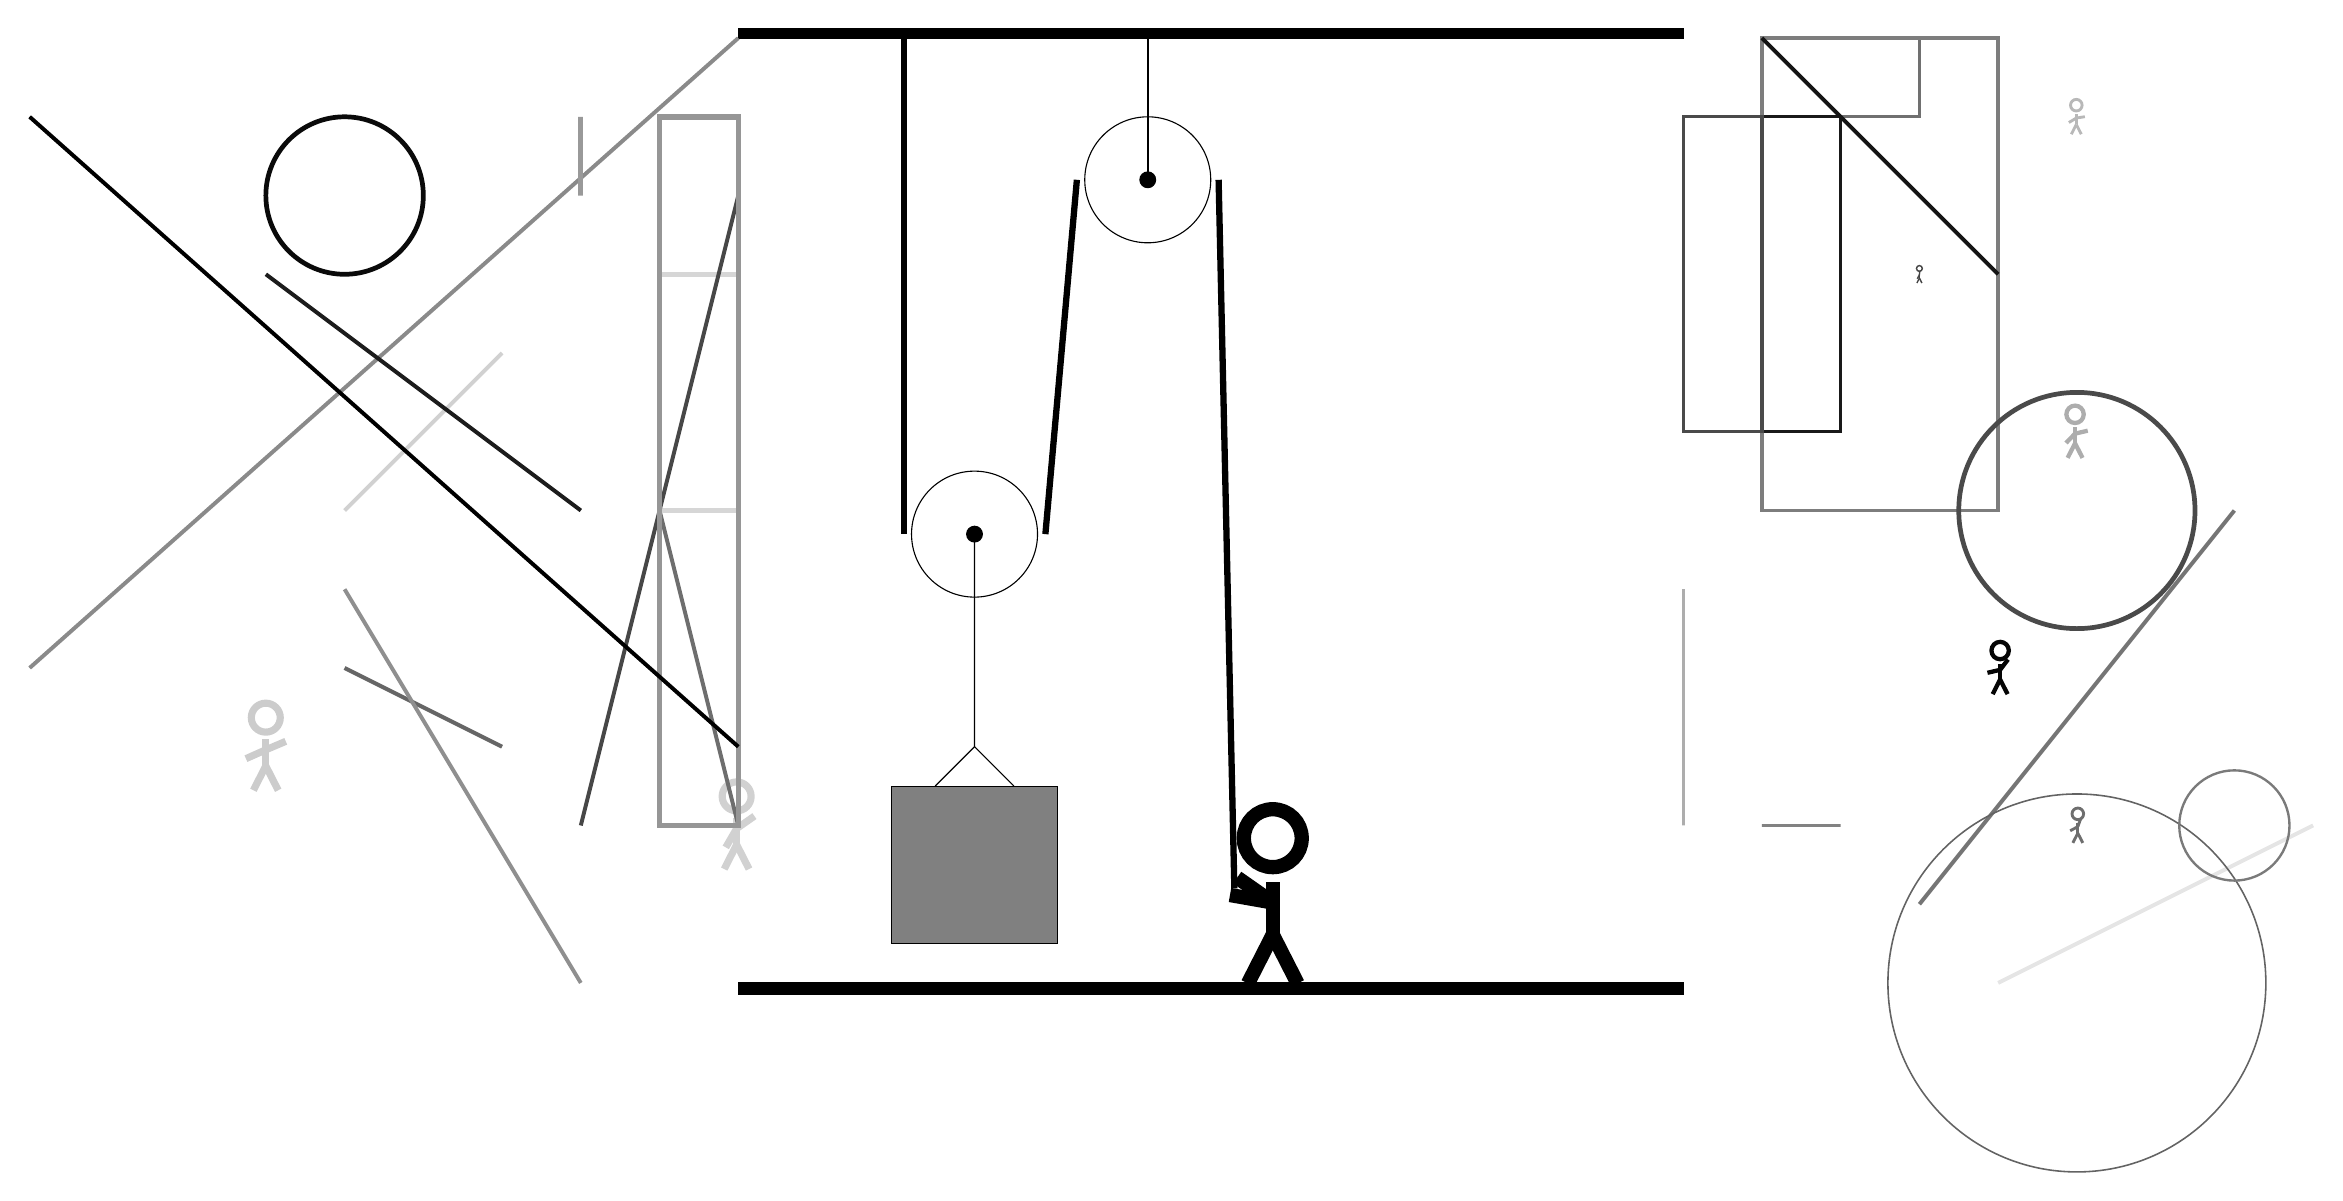
\begin{tikzpicture}
			%%%%% START %%%%%
			
			\draw[fill=black] (-2, 9) rectangle (10, 9.125);
			
			\draw (3.2, 7.2) circle (0.8);
			\draw[fill=black] (3.2, 7.2) circle (0.1);
			\draw[thick] (3.2, 7.2) -- (3.2, 9);
			
			\draw (1, 2.7) circle (0.8);
			\draw[fill=black] (1, 2.7) circle (0.1);
			
			\draw (1, 2.7) -- (1, 0) -- (0.5, -0.5);
			\draw (1, 0) -- (1.5, -0.5);
			\draw[fill=black!50] (-0.05, -0.5) rectangle (2.05, -2.5);
			
			\draw[line width=0.8mm] (0.1, 9) -- (0.1, 2.7);
			\centerarc[line width=0.8mm](1, 2.7)(180:360:0.9);
			\draw[line width=0.8mm](1.9, 2.7) -- (2.3, 7.2);
			\centerarc[line width=0.8mm](3.2, 7.2)(0:180:0.9);
			\draw[line width=0.8mm](4.1, 7.2) -- (4.3, -1.8);
			
			\draw[line width=0.4mm, color=black!56] (11, 9) rectangle (13, 8);
			
			\draw[line width=0.4mm, color=black!90] (12, 4) rectangle (11, 8);
			\draw[line width=0.5mm, color=black!51] (11, 3) rectangle (14, 9);
			\draw[line width=0.5mm, color=black!18](-5, 5) -- (-7, 3);
			\draw [line width=0.6mm, color=black!71](15, 3) circle (1.5);
			\draw [line width=0.6mm, color=black!96](-7, 7) circle (1.0);
			\draw[line width=0.5mm, color=black!60](-7, 1) -- (-5, 0);
			\node[line width=0.5mm, color=black!18] at (-2, -1) {\Strichmaxerl[5][60][35]};
			\node[line width=0.6mm, color=black!20] at (-8, 0) {\Strichmaxerl[5][24][23]};
			\draw[line width=0.5mm, color=black!54](13, -2) -- (17, 3);
			\draw[line width=0.5mm, color=black!57](-2, -1) -- (-3, 3);
			\draw[line width=0.5mm, color=black!21] (-3, 4) rectangle (-3, -1);
			\node[line width=0.3mm, color=black!98] at (14, 1) {\Strichmaxerl[3][13][53]};
			\node[line width=0.3mm, color=black!28] at (15, 8) {\Strichmaxerl[2][31][9]};
			\draw[line width=0.6mm, color=black!16] (-3, 6) rectangle (-2, 3);
			\node[line width=0.6mm, color=black!32] at (15, 4) {\Strichmaxerl[3][46][13]};
			
			\node[line width=0.2mm, color=black!57] at (15, -1) {\Strichmaxerl[2][28][70]};
			\draw[line width=0.3mm, color=black!49] (11, -1) rectangle (12, -1);
			\draw[line width=0.4mm, color=black!32] (10, 2) rectangle (10, -1);
			\draw[line width=0.5mm, color=black!72](-2, 7) -- (-4, -1);
			\draw[line width=0.5mm, color=black!44](-7, 2) -- (-4, -3);
			\draw[line width=0.5mm, color=black!46](-2, 9) -- (-11, 1);
			\draw[line width=0.7mm, color=black!41] (-2, -1) rectangle (-3, 8);
			\node[line width=0.2mm, color=black!73] at (13, 6) {\Strichmaxerl[1][61][85]};
			\draw[line width=0.6mm, color=black!40] (-4, 8) rectangle (-4, 7);
			\draw[line width=0.4mm, color=black!71] (10, 8) rectangle (11, 4);
			\draw[line width=0.5mm, color=black!10](14, -3) -- (18, -1);
			\draw [line width=0.2mm, color=black!61](15, -3) circle (2.4);
			\draw[line width=0.5mm, color=black!100](-2, 0) -- (-11, 8);
			
			\draw [line width=0.3mm, color=black!52](17, -1) circle (0.7);
			\draw[line width=0.5mm, color=black!89](-4, 3) -- (-8, 6);
			\draw[line width=0.5mm, color=black!92](14, 6) -- (11, 9);
			
			\node at (4.7, -1.9) {\Strichmaxerl[10][-35][170]};
			
			\draw[fill=black] (-2, -3) rectangle (10, -3.15);
			
			%%%%% END %%%%%
		\end{tikzpicture}
	\end{figure}	
\end{document}